
\section{The physics} \label{sec:ThePhysics}
In this section, I explain the theoretical framework necessary for understanding and implementing our numerical simulations.

\subsection{Potential-Density Pairs}\label{SEC:potential-density-pairs}

It is intriguing to draw a comparison between 'stellar dynamics' and 'celestial dynamics.' In essence, this involves contrasting the motion of stars within a galaxy with the motion of celestial bodies within our solar system. In the solar system, the gravitational field is known to high precision. Typically, one starts by considering the Sun and then introduces additional complexities as required by the specific problem at hand. For instance, if the goal is to send the James Webb Space Telescope into orbit around the Sun-Earth $L_1$ Lagrange point, a first-order computation does not necessitate the inclusion of all other planets in the system. Similarly, if the aim is to investigate the long-term evolution of comet orbits, one considers the effects of the Sun and Jupiter on the orbit of the comet, perhaps Saturn as well. In essence, the approach entails identifying the most influential bodies in the system and then applying principles derived from the restricted three- or four-body problem.

In the realm of galactic dynamics, the paradigm differs significantly. To begin with, we are dealing with an immense number of stars—billions, to be precise. However, when considering the orbits of bodies within the Galaxy, we need not account for direct star-star interactions. A compelling rationale for this can be found in Chapter 1.2.1 of \citet{2008gady.book.....B}, where the authors demonstrate that direct stellar encounters are exceedingly rare, with their cumulative effects on significantly changing a star's momentum being substantial only after a staggering timescale of 10$^{16}$ years—a duration far surpassing the age of the universe.

As a result, our focus shifts from individual stars to the continuous density distribution of stars throughout the Galaxy. Consequently, the paradigm in galactic dynamics revolves around employing observational evidence to constrain the mass adistribution, ultimately leading to the determination and validation of the gravitational field. This process hinges on arguably one of the most pivotal equations in dynamics, known as Poisson's equation:

\begin{equation}
    \nabla^2 \Phi = 4\pi G \rho.
\end{equation}

To present this equation in a more intuitive fashion, we can shift our focus from examining the Laplacian of the potential to analyzing the divergence of the gravitational field. This is feasible because the gravitational field is 'conservative,' signifying that it arises from the gradient of a scalar-valued function, which is the gravitational potential. In other words, we can express this relationship as: $\nabla \Phi = - \vec{g}$. The negative sign signifies that the gravitational force doesn't act in the direction of the steepest ascent, but rather in the direction of descent. Consequently, through this substitution, Poisson's equation can be reformulated as:
\begin{equation}
    \nabla \cdot \vec {g} = -4\pi G \rho,
\end{equation}
This equation provides a captivating physical insight: if we visualize a gravitational field as a fluid, a mass behaves like a 'sink.' As the density increases, the rate at which this 'matter-fluid' flows toward the mass also intensifies. Moving forward, it's valuable to approach Poisson's equation in integral form, which aids in determining the mass distribution of the gravitational field. This is achieved by initially integrating over a volume and subsequently applying the divergence theorem. The theorem allows us to transition from evaluating the divergence of the gravitational field within a volume to instead considering the flux passing through a surface.

Simultaneously, by performing a volume integral over the density, we can derive the mass profile. The key challenge lies in selecting appropriate integration limits to ensure that the gravitational field and the normal vectors of the chosen surface are consistently parallel. Consequently, the right-hand side of the equation is often treated as:
\begin{equation}
    \int \left(\nabla \cdot \vec{g} \right) dV = \oint \vec{g} \cdot d\vec{S} = g SA.
\end{equation}
Simultaneously, the right hand-side is treated as:
\begin{equation}
    4\pi G \int \rho dV = 4\pi G M_{\textrm{enc}},
\end{equation}
where $M_{\textrm{enc}}$ is the mass enclosed within the same surface. In the end, these two quantities can be related: 
\begin{equation}\label{EQ:force_from_enclosed_mass}
    \vec{g} = \frac{4\pi G M_{\textrm{enc}}}{SA} \hat{n},
\end{equation}
where the unit vector is re-introduced given the symmetry chosen symmetry of the problem. This quickly gives rise to the familiar Keplerian case, when the mass enclosed is a point mass and the equi-potential surface is a sphere, i.e. $SA=4\pi r^2$, and we will have re-derived Newton's law of gravitation: $    \vec{g} = \frac{G M}{r^2} \hat{r}$.


A series of exercises can subsequently be undertaken. If a high degree of symmetry is present, and a chosen density distribution is given, one can straightforwardly determine the gravitational field. Some basic exercises include finding the gravitational field of: a point mass, a uniform sphere, a sphere with increasing mass, an infinitely large sheet, and so on. The reverse approach is also possible, in which one first selects the form of the potential and then applies the Laplacian to deduce the density distribution. An example, and a potential that I employ in my thesis, is the Plummer distribution:

\begin{equation}
\Phi(r|M,b) = \frac{GM}{\sqrt{r^2 + b^2}}.
\end{equation}
This can be understood as a point mass that has been smeared by some characteristic length, $b$. There exists another famous model which applies the same softening principle, the Hernquist: $\Phi(r) = \frac{GM}{r + b}$ \citep{1990ApJ...356..359H}. Additionally one can move to distributions with cylindrical symmetry, an example of a model I employ in my thesis is the Myamoto-Nagai \citep{1975PASJ...27..533M}: 
\begin{equation}
    \Phi\left(R,z|M,a,b\right) = \frac{GM}{\sqrt{R^2 + \left(\sqrt{z^2 + b^2} + a\right)^2}},
\end{equation}
where $a$ is the characteristic disc length, and $b$ is the characteristic disc height. Interestingly, if $a$ is set to zero, a Plummer distribution is recovered. Another important model that I will present here is the Allan-Santillian Halo model. But first, there is an important concept to introduce that is often used as a diagnostic tool for galaxies, known as the 'rotation curve.' In essence, we can measure the net rotation of a galaxy by determining the rotational speed of its constituent stars. A body in a circular orbit has all of its kinetic energy in rotational velocity, and thus the centripetal force counterbalances gravity when $\frac{v_c^2}{r} = g$. We can use EQ.~\ref{EQ:force_from_enclosed_mass} to relate the circular velocity to the enclosed mass, as in the case of spherical symmetry, as:
\begin{equation}
    v_c = \sqrt{\frac{G M_{\textrm{enc}}}{r}}.
\end{equation}
Considering this relationship, and the empirical observation that many external galaxies exhibit nearly constant rotation curves at greater distances, \citet{1986RMxAA..13..137A} proposed a halo potential characterized by mass increasing linearly with distance, resulting in a consistent rotational speed. This concept can be mathematically expressed through the following power law:
\begin{equation}
    M_{\textrm{enc}}\left(r|M_0,\beta,\gamma\right) = \frac{M_{0}\left(r/\beta\right)^{\gamma}}{\left(1+\left(r/\beta\right)\right)^{\gamma-1}}.
\end{equation}
In this formulation, the mass diverges, rendering the model non-physical. Therefore, $M_0$ doesn't represent the total mass but rather serves as a parameter defining the rate at which mass accumulates with increasing distance. On the other hand, $\beta$ denotes a scale length parameter, indicating distances under which mass accumulation is minimal. This potential is referred to as a `halo' potential because it aims to simulate the presence of the dark matter halo enveloping the Galaxy. It's worth noting that, in practice, halos contribute less to the interior of galaxies when compared to visible matter. Another essential consideration is determining the radius at which to truncate the halo. In our article, we adhered to the convention proposed in earlier studies, choosing to truncate it at 100 kpc. This yields the following potential:
\begin{equation}
    \Phi\left(r|M_t,\gamma,\beta,r_\mathrm{c}\right) = -\frac{GM_t}{r} - \frac{GM_t}{\left(\gamma-1\right)\beta}\left.\left[\frac{\left(\gamma-1\right)}{1+\left(r'/\beta\right)^{\gamma-1}} - \ln\left(1+\left(r'/\beta\right)^{\gamma-1}\right)\right]\right|_{r_c}^{r},
\end{equation}
where $r_0$ is the truncation radius, $\gamma$ is the power parameter whose best fit value was found to be 2.02, and $M_t$ is the total mass. These values for all of the can be found in Table 1 of \citet{2023A&A...673A..44F}. 

\subsubsection*{The Laplacian is a linear operator}
It is important to note that the Laplacian is a linear operator, i.e. $\nabla^2\left(a_0\Phi_0 + a_1\Phi_1\right) = a_0\nabla^2\Phi_0 + a_1\nabla^2 \Phi_1$. Likewise, the right hand-side of Poisson's equation is multiplication, which is a linear. Therefore both the total potential and the total density of a system can be described as a sum of simpler parts:

\begin{equation}
    \nabla^2 \left(\Phi_0 + \Phi_1 + \dots + \Phi_N \right) = 4\pi G \left(\rho_0 + \rho_1 + \dots + \rho_N \right).
\end{equation}
This is fundamental when creating models and allows us to dissect the Milky Way into parts based on different pieces of observational motivation. This is what is done by many Galactic potential models: \citet{1991RMxAA..22..255A}, \citep{2017MNRAS.465...76M}, and lastly, the potential model that we employ this this work, \citet{2017A&A...598A..66P}. This paper presents two models and compares them the older model of \citet{1991RMxAA..22..255A}. One of the models consists of a small central bugle described by a Plummer, two Miyamoto-Nagai disks, and a Allen-Santillian halo. The second model consits of two discs and the dark matter halo only. 

\subsection{Distribution Function Sampling} \label{sec:DistributionFunctionSampling}

In this thesis, my objective is to simulate the integration of star-particles' orbits within Galactic globular clusters and observe their escape, forming tidal tails. A crucial aspect is the accurate establishment of initial conditions for these star-particles. To achieve this, I have drawn inspiration from chapter 4 of \citet{2008gady.book.....B}, which have informed this section. To begin, the distribution of stars within the system of interest is described by a six-dimensional distribution function over the phase space variables, denoted as $f\left(\vec{x},\vec{v}\right)$. Given that this is a distribution function, it is inherently normalized. Consequently, when integrated over the phase space variables, the result is equal to 1: $\mathcal{P}=\int f\left(\vec{x},\vec{v}\right) d^3\vec{x}d^3\vec{v}=1.$ Another assumption that is made in DF modeling is that the phase-space volume is constant. i.e. $\frac{d f}{dt}=0$. By applying the derivative and chain rule, we obtain:
\begin{equation}
    \frac{df}{dt} = \frac{\partial f}{\partial t} + \frac{\partial f}{\partial \vec{x}}\cdot\frac{d\vec{x}}{dt}+\frac{\partial f}{\partial \vec{v}}\cdot\frac{d\vec{v}}{dt} = 0.
\end{equation}
In practice, this equation is stating that stars are not being created or destroyed, which is not strictly true but satisfactory for our purposes. For instance, stars in globular clusters are very light and not massive enough to go super nova. Additionally, stars within globular clusters are old, and gas-less thus are not creating stars. 

Next, this equation is manipulated for various physical configurations, i.e. if this mass distribution is spherical, or if the velocity of the stars are \textit{isotropic} (equally random in all directions), or if there is anisotropy, i.e. a correlation between the velocities of stars. In my thesis thus far, I have analyzed one of the simplest cases, an Isotropic Plummer distribution. To do this, I have taken the result that the distribution function depends only on the energy as:
\begin{equation}\label{EQ:plummerDF}
    f\left(E\right)\propto E^{-7/2},
\end{equation}
Here, the energy, denoted as $E$, combines the kinetic and potential energies, and it is expressed as: $E=\frac{1}{2}v^2 + \frac{GM}{\sqrt{r^2 + b^2}}$. Armed with this knowledge, we can formulate a set of initial conditions for a globular cluster, taking into account its specific mass and characteristic radius.

\subsubsection*{Inverse Transform Sampling}
Inverse transform sampling is a highly practical technique for generating a set of discrete realizations from any probability density function. In theory, it operates as follows: Let $\mathcal{F}$ be the cumulative distribution function (CDF) of a given probability density function, denoted as $f$:
\begin{equation}
    \mathcal{F}\left(x\right) = \int_{-\infty}^{x} f\left(x'\right)dx'.
\end{equation}
The probability of drawing any number $x$, to be less than $x_0$, is the value of the CDF at $x$:
\begin{equation}
    \mathcal{P}\left(x < x_0\right) = \mathcal{F}\left(x\right).
\end{equation}
Since CDFs are monotonically increasing and one-to-one with the independent variable, we can substitute:
\begin{equation}
 \mathcal{P}(F(x)<F(x_0)) = \mathcal{P}(x<x_0).
\end{equation}
Now we may introduce a random variable $Y$, whose value is equally probably between [0,1], which is described by a DF of:
\begin{equation}
f(y) = \begin{cases} 1 & \text{if } y \in [0,1] \\ 0 & \text{otherwise} \end{cases}
\end{equation}    
We can substitute, stating that the probability of drawing a uniform random value between [0,1] is the same probability of drawing a value $x$ as being less than the value of interest: $x_0$.
\begin{equation}
    \mathcal{P}\left(Y<\mathcal{F}(x_0)\right) = \mathcal{P}(x<x_0).
\end{equation}
Again, since the CDF and $x$ are monotonically related and one-to-one, we can apply the inverse transform to the left hand side:
\begin{equation}
\mathcal{P}\left(\mathcal{F}^{-1}(Y)<x_0\right) = \mathcal{P}(x<x_0),
\end{equation}
which in turn leads to the desired result that:
\begin{equation}
    \mathcal{F}^{-1}\left(Y\right) = x.
\end{equation}
In practice, you can visualize this equation as follows: imagine plotting any CDF against the independent variable, and then randomly drawing horizontal lines with heights between [0,1] from negative infinity. Observe where these lines intersect the CDF, which determines the corresponding $x$ values. 

For instance, consider the Plummer sphere. We wish to sample this distribution to find a set of initial conditions for $N$ particles. The CDF of the normalized mass distribution is as shown in Fig.~\ref{fig:inverse-transform-sampling}. The fraction of the total enclosed mass, denoted as $M_X$ as a function of distance scaled to the characteristic length, $r_X = r/b$, is:
\begin{equation}
    M_X = \frac{r_X^3}{\left(1+r_X^2 \right)^{3/2}}.
\end{equation}
The plot shown in Fig.~\ref{fig:inverse-transform-sampling} has a scale radius of 10. 

\begin{figure}
    \centering
    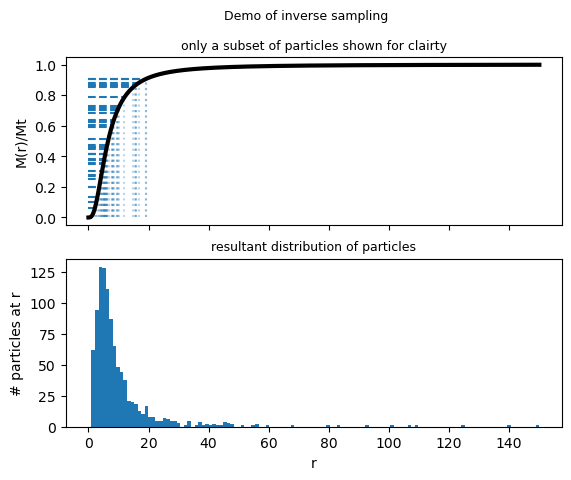
\includegraphics[width=0.75\linewidth]{images/inverse-transform-sampling.png}
    \caption{An example of inverse transform sampling. The CDF shown in the top panel is the enclosed mass of a Plummer sphere, normalized by its total mass. The horizontal blue lines are sampled from a uniform distribution, using the function \texttt{np.random.rand()} from Python's  library \texttt{numpy}, and are traced to intersect the CDF. }
    \label{fig:inverse-transform-sampling}
\end{figure}

Applying inverse transform sampling to this mass distribution provides the radial distances from the center of the system. Next, we need to find the angular positions on the unit sphere. One may naively attempt to uniformly sample the polar and azimuthal angles, $\theta,\phi$, however this would incorrectly bunch up points at the poles. One must instead consider a DF in which sampling equally probable in all areas. The argument is as follow, first: $\int f dA' = 1$ where we are integrating over a unit sphere. We know that $\int dA = 4\pi$, thus, $f dA' = (1/4\pi) dA$. Note that $dA'$ does not equal $dA$. Next, on a sphere the infinitesimal surface area is $dA = \sin(\theta)d\theta d\phi$. We can now related this to the DF, $f=(1/4\pi)\sin(\theta)$ and $dA' =d\theta d\phi$. This DF is used to find the CDF, which is then used to randomly sample the angles. Notice that it does not depend on $\phi$, which is thus sampled from a uniform DF, which is a linear CDF that ranges [0,1] and runs over [0,$2\pi$].

Lastly, sampling the velocities is not independent from the from the position, so we must consider the conditional DF: $f(v|r)$ from Eq.~\ref{EQ:plummerDF}. The number density of particles at a point, $\vec{x}$, is found by integrating the velocities, i.e. $N(\vec{x})=\int f(\vec{v}|\vec{x})d^3\vec{v}$. Note that another way of writing a probability density function, is $f'=\frac{dN}{dv}$. Also note that because we are assuming the velocities are equally random in all directions, we may find $\frac{dN}{dv}$ by integrating then total DF and then differentiate with respect to $v$:

\begin{equation}
    \frac{dN}{dv} = \frac{d}{dv}\int f(\vec{v}|\vec{x}) (v\sin\theta'd\phi')(vd\theta')(dv) = 4\pi v^2 f(v|\vec{x}),
\end{equation}
which gives the number density per particle speed. Note that the angles here are not in physical space but rather velocity space. Lastly, to construct the CDF of this DF, we must know what the proper limits are. The speeds available to this particle range from zero to the escape speed, which is $v_{esc}=\sqrt{2\Phi(r)}$. Thus, the CDF is:
\begin{equation}\label{EQ:CDF-velocities}
    CDF(v) = C \int_0^{v<v_{esc}} 4\pi v^2 f(v|\vec{x}) dv,
\end{equation}
where $C$ is a normalization constant. In practice, we ignore this constant because for each particle position, we find the non-normalized CDF and then divide by the final value to normalize it. This process is visualized in Fig.~\ref{fig:cdf-velocities}. Once the speeds are found, the orientations of the velocity vectors can by found by randomly sampling x,y,z values from uniform random distributions between [-1,1] and then re-normalizing the resultant vector and multiplying it by the final speed. 

\begin{figure}
    \centering
    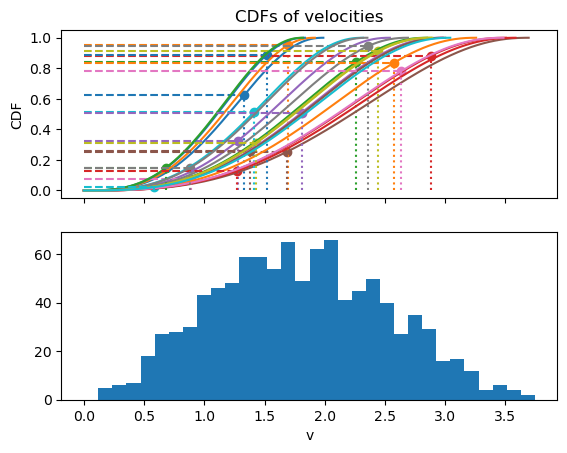
\includegraphics[width=0.75\linewidth]{images/cdf-velocities.png}
    \caption{An example of inverse transform sampling of the initial velocities. Each CDF is created per particle, since we are sampling the velocities given an initial position. The CDF's have the functional forms specified by Eqs.~\ref{EQ:plummerDF}~and~\ref{EQ:CDF-velocities}.}
    \label{fig:cdf-velocities}
\end{figure}


\subsection{Tidal Forces and the Restricted Three Body Problem}

With the potential-density pairs discussed in section~\ref{SEC:potential-density-pairs} and a method in place for generating initial positions within a sphere of star-particles, the stage is set to address a fundamental question: \textit{What causes stars to escape from globular clusters?}

\subsubsection*{Tidal Forces}
As any good physicist would do, we will first solve a simpler problem and draw insights from it while considering the more complex problem at hand. Instead of considering the Galaxy exerting a force on a globular cluster, consider the gravitational force from a point mass acting on three points along a line: $r-\delta r$, $r$, $r+\delta r$, where $\delta r<< r$. We can perform a Taylor expansion to approximate the force to second order at the interior and exterior points.   
\begin{equation}
    F_{inside}=-\frac{GMm}{\left(r-\delta r\right)^2} \sim -\frac{GMm}{r^2}\left[1+\frac{2\delta r}{r}\right]
\end{equation}

\begin{equation}
    F_{outside}=-\frac{GMm}{\left(r+\delta r\right)^2} \sim -\frac{GMm}{r^2}\left[1-\frac{2\delta r}{r}\right]
\end{equation}
When describing these forces relative to the center of mass of the body located at $r$, we subtract the force vector upon the center and see that the opposite sides of the body are being ripped away from the center with a force:

\begin{equation}
    F_{\mathrm{tidal}}\sim 2GMm \frac{\delta r}{r^3}.
\end{equation} 
By positioning an extended body in a gravitational field where the gravitational pull is stronger closer to the center than at a greater distance, it results in tidal forces. It's worth noting the functional form of the tidal force originating from the center of mass of the object: this force increases linearly with distance from the center of the object. Additionally, it follows an inverse-cubed relationship between the distance to the host, making it considerably weaker than the gravitational force. 

This is a suitable qualitative comparison. Even though the galactic gravitational field is not Keplerian, as in the previous example, it's well-established that the gravitational field still exhibits a gradient and is more pronounced toward the center. Furthermore, globular clusters are inherently extended, spherical bodies. Therefore, based on the previous example, we anticipate that globular clusters will undergo deformation along the radial direction, with those farther from the center cluster experiencing more significant deformation than those situated farther away.


\subsubsection*{The circular restricted-planar three body problem}

Another simpler system to draw parallels with, as we aim to establish a theoretical conceptual framework, is the restricted three-body problem. In this scenario, we analyze two masses that mutually affect each other and a third particle that doesn't exert any gravitational force but is influenced by the other two bodies. A well-known instance of this is the Sun-Earth-Spacecraft setup. While the theory for this section will be further elaborated in the thesis, my objective here is to offer a broad overview of the mechanics.

In essence, when examining the restricted three-body problem, we further simplify this scenario. Initially, we assume that the two larger bodies are in circular orbits around the center of mass. This enables us to establish a non-inertial reference frame that rotates at a constant angular velocity, matching that of the two larger bodies. Subsequently, we analyze the situation in which the third particle orbits within the same plane as the two massive bodies. Despite these simplifications, we can derive potent physical tools for comprehending tidal phenomena. Firstly, we begin by formulating the Lagrangian of the third particle:
\begin{equation}
    \mathcal{L}_{\mathrm{inertial frame}} = T(\dot{x},\dot{y},\dot{z}=0)-U(x,y,z=0,t)
\end{equation}
When we analyze the problem within an inertial frame, the potential energy is time-dependent motion since the larger two bodies are in motion with respect to the reference frame, leading to increased complexities. Consequently, we transition to a non-inertial reference frame, rotating at the same angular velocity as the two massive bodies. Given our simplification of the problem to circular orbits, the massive bodies remain fixed at points along the x-axis. While this approach eliminates the time dependence of the potential energy, it introduces a spatial dependence to the kinetic energy:
\begin{equation}
    \mathcal{L}_{\mathrm{rotating frame}} = T(x,y,z=0,\dot{x},\dot{y},\dot{z})-U(x,y,z=0)
\end{equation}
Recall the two-body problem, where we introduced polar coordinates and observed that the kinetic energy also depends on the spatial coordinate, expressed as $(1/2)m\left(\dot{R}^2 +(R\omega)^2 \right)$. To delve deeper into the problem, we shifted this spatial dependence to the potential energy, giving rise to an \textit{effective} potential energy. The same approach is applied to the three-body problem. In this case, we seek locations where the effective potential exhibits critical points. The critical points of the effective potential in the three-body problem are referred to as the \textit{Lagrange points}.


Much like the two-body problem, the three-body problem exhibits distinct categories of orbits based on the total energy. When the total energy is positive, bodies follow hyperbolic orbits; zero energy results in parabolic orbits; negative energy leads to bounded eccentric orbits, and the minimum energy corresponds to circular orbits. Just as in the two-body problem, the three-body problem can be subdivided into different ``realms'' of possible orbits based on the total energy.

In one of these realms, a particle is initially bound to the less massive secondary. It can transition to having its dynamics dominated by the primary body if it possesses a certain level of energy. This transition from being influenced by the secondary to the primary occurs at the \textit{first Lagrange point}. To locate this point, one sets the effective potential equal to zero for a particle along the x-axis in the rotating frame. Remarkably, determining the position of the Lagrange point involves solving a quintic polynomial for which no exact analytic solution exists. Consequently, the location of the Lagrange point is always reported as an approximation.


Another intriguing concept that arises from this analysis is the \textit{Hill} sphere, which can be defined as the sphere encompassing the secondary body within which its gravitational force prevails in influencing the motion of a test particle. Mathematically, this sphere can be expressed as:
\begin{equation}
    r_h = a\left(\frac{m_1}{3\left(m_0+m_1\right)}\right)^{1/3},
\end{equation}
where $a$ is the semi-major axis of the orbit between the two bodies, and there masses are $m_0$ and $m_1$.

\subsection{Phase-Mixing}

Another important concept that will serve to interpret the results is \textit{phase-mixing}.\footnote{Chapter 18 of \url{galaxiesbook.org} has largely inspired this discussion.} Phase-mixing occurs when we an initial distribution of points in phase-space about some location, $r,v$ with some spread or \textit{dispersion}, $\delta r, \sigma_{v}$, naturally spread over time and eventually uniformly distribute themselves over all possible configurations allowed by the system. A good way to estimate the time scale over which this occurs is to look at the maximum difference in frequencies between two particles complete phase space orbits: 

\begin{equation}
    \tau_{\textrm{phase-mixing}} = \frac{2\pi}{\Delta f}.
\end{equation}
Again, to gain physical insight, we can look to the Kerplerian case for some quick estimates. From Kepler's third law, we know the relationship between orbit period and the semi-major axis of an orbit: $T_{\textrm{dyn}}^2\propto a^3$. We can estimate the difference in frequencies by studying the orbits of two points, $r+\delta r$ and $r-\delta r$. This would then lead to:
\begin{equation}
    \Delta f \propto \left(\left(r+\delta r\right)^3 - \left(r-\delta r\right)^3\right).
\end{equation}
Through performing two Taylor expansions by assuming that $\delta r << r$ and substituting $T_{\mathrm{dyn}}$ for $r^3$, we arrive to the relationship that:
\begin{equation}
    \tau_{\textrm{phase-mixing}} \approx T_{\mathrm{dyn}}\left(1-6\frac{\delta r}{r}\right).
\end{equation}
For the case of the globular clusters, a typical scale size is five parsecs, while their orbital radii are on the scale of kilo-parsecs. This large difference in size renders the characteristic time for phase mixing to be approximately equivalent to a dynamical time, $\tau_{\textrm{phase-mixing}} \approx T_{\mathrm{dyn}}$. 

While this quick analysis gives us some powerful insight, this $\tau_{\textrm{phase-mixing}}$ time is an under estimate. This is largely due to the fact that the gravitational pull of the globular cluster keeps its star close. Thus, the real phase mixing will be larger than the dynamical time. Nonetheless, this serves as a first order guide. We expect that clusters whose $T_{\mathrm{dyn}}$ is much less than the duration of the simulation will have totally mixed tidal debris. Whereas those with $T_{\mathrm{dyn}}$ is comparable or less than the total simulation time will not have phase-mixed debris and thus the escaped star particles will still reside near the cluster.

